\documentclass[12pt,a4paper]{article}
\usepackage[spanish,es-tabla]{babel}
\usepackage{listings}
\usepackage[colorlinks=false]{hyperref}
\usepackage{graphicx}
\usepackage{multirow}
\usepackage{amsmath}
\usepackage{textcomp}
\usepackage{algorithm}
\usepackage{caption}
\usepackage{algpseudocode}
\usepackage{amsmath}
\usepackage{amssymb}

\captionsetup[algorithm]{labelsep=colon, name=Algoritmo}
\captionsetup{justification=centering}

\renewcommand\vec[1]{\ifstrequal{#1}{0}{\ensuremath{\mathbf{0}}}{\ensuremath{\boldsymbol{#1}}}}

\renewcommand{\abstractname}{Resumen}
\def\tablename{Tabla}

\begin{document}

\begin{titlepage}
  \centering
  \vspace*{0.5cm}
  
\includegraphics[height=2.2cm]{resources/itba.png}\par
  \vspace{0.6cm}
  {\Large \textbf{Instituto Tecnológico de Buenos Aires}}\par
  \vspace{1.6cm}

  {\LARGE \textbf{Trabajo Práctico N°2}}\par
  \vspace{0.3cm}
  {\Large \textbf{72.25 Simulación de Sistemas}}\par
  \vspace{0.3cm}
  {\Large Autómatas Celulares}\par
  \vspace{1.8cm}

  \begin{flushleft}
    \textbf{Grupo:} 10 \par
    \vspace{0.6cm}
    \textbf{Integrantes:}\par
    Barnatán Martín Alejandro (64463) \\
    \quad \href{mailto:mbarnatan@itba.edu.ar}{mbarnatan@itba.edu.ar}\par
    \vspace{0.3cm}
    Maurottolo Quiroga Ignacio Martín (64611)\\
    \quad \href{mailto:imaruottoloquiroga@itba.edu.ar}{imaruottoloquiroga@itba.edu.ar}\par
    \vspace{0.3cm}
    Pedemonte Berthoud Ignacio (64908) \\
    \quad \href{mailto:ipedemonteberthoud@itba.edu.ar}{ipedemonteberthoud@itba.edu.ar}\par
    \vspace{0.6cm}
    \textbf{Fecha de Entrega:} 29 de Agosto de 2025\par
  \end{flushleft}

  \vfill

  \begin{flushright}
    \centering
    2C - 2025
  \end{flushright}
\end{titlepage}
\newpage

\tableofcontents
\newpage

\begin{abstract}
El presente informe consta del trabajo realizado en el contexto del Trabajo Práctico N°2 para la materia Simulación de Sistemas en el Instituto Tecnológico de Buenos Aires. El mismo consistió en el estudio de la implementación computacional del modelo de Vicsek para sistemas de partículas autopropulsadas que interactúan en un plano bidimensional. Se estudiaron variaciones en los parámetros principales del modelo, como la densidad de partículas y la intensidad del ruido, evaluando sus efectos sobre la dinámica y el grado de orden del sistema.
\end{abstract}

\section{Introducción}

Para la realización del trabajo, se tomó como base el paper \textit{Novel Type of Phase Transition in a System of Self-Driven Particles} de \textit{Tamás Vicsek, András Czirók, Eshel Ben-jacob, Inon Cohen y Ofer Shochet} que considera un conjunto de partículas puntuales que se mueven en un plano bidimensional con velocidad constante, y que en cada paso temporal ajustan su dirección de movimiento para alinearse con la orientación promedio de sus vecinos dentro de un radio de interacción, incorporando además una perturbación aleatoria asociada al ruido del sistema. Mediante este modelo, se puede realizar un estudio de fenómenos colectivos presentes en la naturaleza, como es el caso de las bandadas de pájaros, donde a partir de interacciones locales simples emergen patrones globales de alineamiento y organización.\\

Para caracterizar el comportamiento del sistema se definieron observables, siendo el más relevante el parámetro de orden $v_a$, que mide el grado de alineamiento colectivo de las partículas. El análisis de su evolución temporal, así como de su valor promedio en el estado estacionario, permite estudiar cómo influyen parámetros de entrada como la densidad de partículas y la intensidad del ruido en la dinámica y en la transición entre estados desordenados y ordenados.\\

Tal como en el estudio presentado por \textit{Vicsek}, las simulaciones se realizan en un espacio bidimensional dentro de una celda cuadrada de lado $L$, bajo condiciones periódicas de contorno. Esto significa que una partícula que atraviesa un borde de la celda vuelve a ingresar por el lado opuesto, evitando efectos de borde y garantizando una densidad constante. Las partículas se modelan como puntos que se desplazan de manera continua en el plano, lo que define al modelo como un autómata celular off-lattice. La dinámica se desarrolla en tiempos discretos: en cada intervalo $\Delta t$, todas las partículas actualizan simultáneamente su dirección y su posición.\\


El sistema contiene cinco variables principales que determinan su comportamiento:

\begin{itemize}
    \item $N$: Cantidad de partículas del sistema.
    \item $L$: Longitud del lado de la celda cuadrada que delimita el espacio bidimensional de simulación.
    \item $r_c$: Radio de interacción de las partículas.
    \item $v$: Módulo de la velocidad de la partícula.
    \item $\eta$: Intensidad del ruido, que introduce una perturbación aleatoria en la dirección de movimiento de cada partícula.
\end{itemize}

A partir de dichas variables, se puede definir también la densidad del sistema, que se obtiene mediante

\begin{equation}
    \label{densidad}
    \rho = \tfrac{N}{L^2}.
\end{equation}

El modelo se basa principalmente en dos ecuaciones, la Ec.~\eqref{posicion} que determina la posición de la partícula $i$ y la Ec.~\eqref{angulo} que define la actualización de su dirección de movimiento.

\begin{equation}
    \label{posicion}
    x_i(t+1) = x_i(t) + v_i(t) \Delta t
\end{equation}

donde $x_i(t)$ representa la posición de la partícula $i$ en el instante $t$, $v_i(t)$ es su vector de velocidad y $\Delta t$ es el intervalo temporal entre dos actualizaciones sucesivas.

\begin{equation}
    \label{angulo}
    \theta(t+1) = \langle \theta(t) \rangle_r+ \Delta \theta
\end{equation}

donde $\theta_i(t+1)$ es el ángulo de la partícula $i$ en el instante $t+1$, $\langle \theta(t) \rangle_r$ corresponde al promedio de las orientaciones de todas las partículas ubicadas dentro de un radio de interacción $r$ alrededor de $i$, y $\Delta \theta$ es un término de ruido aleatorio tomado de una distribución uniforme en el intervalo $[-\eta/2, \eta/2]$.\\

La dirección promedio $\langle \theta(t) \rangle_r$ se calcula a partir de los senos y cosenos de los ángulos de las partículas vecinas, mediante

\begin{equation}
    \label{mean_angle}
    \langle \theta(t) \rangle_r = \arctan \left( \frac{\langle \sin \theta(t) \rangle_r}{\langle \cos \theta(t) \rangle_r} \right)
\end{equation}

donde $\langle \sin \theta(t) \rangle_r$ y $\langle \cos \theta(t) \rangle_r$ representan los promedios de los senos y cosenos de las direcciones de las partículas dentro del radio de interacción $r$. 

\section{Implementación}

La implementación del modelo se realizó en \textbf{Python 3} aprovechando \texttt{NumPy} para el cálculo vectorizado y \texttt{Matplotlib} para la generación de animaciones y gráficos. El proyecto se estructura en módulos independientes (Fig.~\ref{estructura}): 
\texttt{vicsek.py} (modelo y utilidades numéricas), 
\texttt{simulate.py} (corridas y persistencia),
\texttt{visualizer.py} (animaciones),
\texttt{graphs.py} (observables y figuras) y 
\texttt{simulation\_processing.py} (lectura y post-proceso de resultados).

\begin{figure}[h]
\centering
\begin{minipage}{0.78\linewidth}
\small
\begin{verbatim}
sds-tp2/
 |-- data/
 |-- graphs.py
 |-- simulate.py
 |-- simulation_processing.py
 |-- vicsek.py
 |-- visualizer.py
\end{verbatim}
\end{minipage}
\caption{Estructura del repositorio utilizada para el TP.}
\label{estructura}
\end{figure}

\subsection{Arquitectura y Módulos}

Como se puede visualizar en la Fig.~\ref{estructura}, el código se organizó en distintos módulos de \texttt{Python}, cada uno con una responsabilidad diferente:

\begin{itemize}
    \item \textbf{vicsek.py}: Implementa el modelo de Vicsek. Incluye la definición de parámetros y estado, así como las funciones para inicializar el sistema, calcular el parámetro de orden y avanzar la simulación paso a paso.
    
    \item \textbf{simulate.py}: Permite ejecutar corridas completas de la simulación y guardar los resultados en archivos. De esta forma los datos quedan disponibles para ser analizados posteriormente.
    
    \item \textbf{simulation\_processing.py}: Lee los resultados guardados y reconstruye las trayectorias y observables de una simulación para facilitar el análisis.
    
    \item \textbf{visualizer.py}: Genera animaciones de la dinámica del sistema a partir de los datos simulados, mostrando tanto las posiciones y direcciones de las partículas como la evolución temporal del parámetro de orden.
    
    \item \textbf{graphs.py}: Produce gráficos comparativos de los observables, por ejemplo la evolución del parámetro de orden para distintos valores de ruido o densidad.
\end{itemize}

En conjunto, esta arquitectura permite separar la simulación del análisis y la visualización, ya que primero se ejecuta y se guarda la dinámica para su animación, y luego se procesan los datos para producir los gráficos. El flujo se puede observar en el diagrama presentado en la Figura

\begin{figure}[ht]
    \centering
    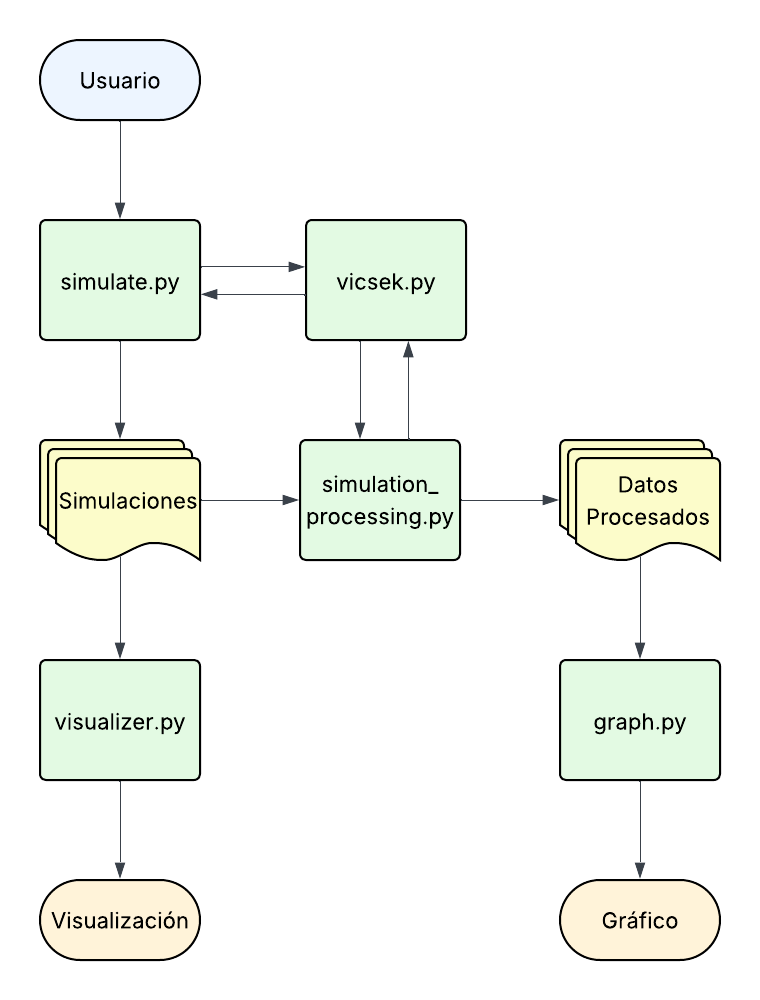
\includegraphics[width=6cm]{resources/diagrama-uml.png}
    \caption{Diagrama de flujo de la arquitectura implementada.}
    \label{diagrama-uml}
\end{figure}


\subsection{Algoritmo}

La dinámica se implementa en tiempos discretos $\Delta t=1$, al igual que en el paper mencionado, y con velocidad constante $v$. En cada paso se:
(i) determinan vecinos dentro de $r_c$ usando \textbf{Cell Index Method}, tomando el algoritmo desarrollado en el Trabajo Práctico N°1; 
(ii) calcula el ángulo promedio de vecinos; 
(iii) agrega ruido uniforme $\Delta\theta$; 
(iv) actualizan direcciones y posiciones aplicando condiciones periódicas.\\

El algoritmo ejecutado en cada paso (o step) de la simulación es el Algoritmo~\ref{algoritmo}. El método \texttt{cell\_index\_method} tomado del trabajo previo, retorna, para cada partícula, una lista con los índices de todas aquellas que se encuentran dentro de su radio de interacción $r_c$. De esta manera, el resultado es una estructura de listas en la que la posición $i$ contiene los vecinos de la partícula $i$. 

\begin{algorithm}
\caption{Paso de simulación (Vicsek)}
\begin{algorithmic}[1]
\State Generar ruido aleatorio para cada partícula
\State Calcular vecinos de cada partícula con Cell Index Method
\For{cada partícula $i$}
    \State ánguloPromedio $\gets$ promedio(ángulo de $i$ y sus vecinos)
\EndFor
\State nuevaDirección $\gets$ ánguloPromedio + ruido
\State Calcular velocidades $(v_x, v_y)$
\State Actualizar posiciones con condiciones periódicas
\State \Return nuevo estado
\end{algorithmic}
\label{algoritmo}
\end{algorithm}

\subsection{Formato de Datos y Reproducibilidad}

Cada ejecución del modelo se guarda en \texttt{data/simulations/<nombre>/} con:
\begin{itemize}
  \item \texttt{static.txt}: parámetros y longitud de la ejecución (una línea por valor)\\
\texttt{\small N\\L\\v\\r\\eta\\T}
  \item \texttt{t.txt} (\(t=0,\dots,T-1\)): $N$ líneas, cada una con \texttt{x\ y\ \(\theta\)} de una partícula en el tiempo $t$.
\end{itemize}

El módulo \texttt{simulation\_processing.py} reconstituye las trayectorias y calcula $v_a(t)$ progresivamente. Esto luego es reproducible gracias a la \texttt{seed} en \texttt{VicsekParams}.

\section{Simulaciones}

En las simulaciones realizadas para el estudio del modelo, se fijaron ciertos valores para todos los casos, tomando como referencia el paper citado previamente:
\begin{itemize}
    \item $r_c = 1$
    \item $v = 0.03$
\end{itemize}

Por otro lado, se tomaron variables para ajustar el estudio al caso particular y al observable en consideración:
\begin{itemize}
    \item $N$: Cantidad de partículas.
    \item $L$: Tamaño de la celda.
    \item $\eta$: Ruido.
    \item $T$: Cantidad de frames.
\end{itemize}

Nótese que otro parámetro importante variable es la densidad $\rho$, a partir de los valores de $N$ y $L$ tomando la Ec.~\eqref{densidad}. A continuación, se detallan las simulaciones realizadas para su posterior visualización y/o gráfico.

\subsection{Simulaciones para Animaciones}
\label{simulaciones-para-animaciones}

En primer lugar, se realizaron simulaciones básicas con el fin de presentar una posterior animación del sistema y del algoritmo de actualización en cada paso. Para esto, se tomaron los siguientes valores:
\begin{itemize}
    \item $N = 300$
    \item $L = 5$
    \item $T = 300$
\end{itemize}

Para obtener un análisis más profundo, se decidió variar el parámetro de ruido $\eta$, haciendo que tome valores de $0.1$, $2$ y un valor aproximado a $2\pi$ ($\eta=6.28$). El objetivo fue tener primero un caso de orden con un valor de ruido bajo, luego uno más intermedio para analizar su evolución y finalmente un valor que genere un régimen desordenado. Cabe recordar que como el ruido angular se toma uniforme en $[-\eta/2,\eta/2]$, al llegar a $\eta=2\pi$ significa que cada partícula puede recibir cualquier ángulo posible en $[-\pi,\pi]$.\\

Adicionalmente, se realizó una simulación con un tamaño de celda mayor, fijando $L=25$ y manteniendo el resto de los parámetros constantes, en particular $\eta=0.1$. Este cambio implica una reducción de la densidad de partículas, ya que $N$ se mantuvo fijo. El objetivo de esta simulación extra fue analizar el efecto de una menor densidad en la dinámica colectiva y en la formación de estructuras coherentes dentro del sistema.

\subsection{Evolución Temporal del Observable}
\label{evolucion-temporal-del-observable}

El observable definido para este estudio es el parámetro de orden $v_a(t)$, que mide el grado de alineamiento de las partículas en función del tiempo. Se define de la siguiente manera:
\begin{equation}
    v_a = \frac{1}{Nv} \left|\sum_{i=1}^{N} \vec{v_i} \right|
\end{equation}

El valor de este parámetro tiende a cero cuando hay un desorden total, y tiende a uno cuando hay una mayor polarización de las partículas.\\

Para establecer en qué tiempos se deben tomar los promedios para calcular el valor escalar (válido) del observable, se realizó una simulación con los siguientes valores para las variables:
\begin{itemize}
    \item $N=2000$
    \item $L=10$
\end{itemize}

En el caso de $\eta$, se tomaron los valores $0.1$, $0.5$, $1.0$, $2.0$, $4.0$ y $6.0$, con el fin de establecer un amplio rango de estudio.

\subsection{Relación entre el Ruido del Sistema y el Observable}
\label{curva-input-vs-observable}

Con el objetivo de analizar la relación entre el parámetro de entrada $\eta$ (ruido) y el observable $\overline{v_a}$ (polarización promedio en régimen estacionario), se realizaron simulaciones adicionales variando sistemáticamente el valor del ruido tal que $
\eta \in \{0.1,\;0.5,\;1.0,\;2.0,\;3.14,\;4.7,\;6.28\}
$.\\

Para cada valor de ruido se ejecutaron 5 combinaciones distintas de $N$ y $L$, manteniendo constante la densidad del sistema en $\rho = 4$:
\begin{itemize}
    \item $N=64$, $L=4$
    \item $N=100$, $L=5$
    \item $N=400$, $L=10$
    \item $N=676$, $L=13$
    \item $N=900$, $L=15$
\end{itemize}

En total, se llevaron a cabo 35 simulaciones, cada una con una duración de $T=1000$ pasos. Tal como se discutió en la Subsección~\ref{evolucion-temporal-del-observable}, se descartó el estado transitorio inicial equivalente a $0.3T$, de modo que el valor reportado $\overline{v_a}$ corresponde exclusivamente al promedio temporal calculado en el régimen estacionario.\\

Para cada condición de ruido $\eta$ se obtuvo la curva $\overline{v_a}$ vs.\ $\eta$, acompañada de sus barras de error. Estas últimas se calcularon como el desvío estándar de los valores de $v_a(t)$ en la región estacionaria, reflejando así las fluctuaciones temporales del observable en torno a su valor medio.\\

Sea $\{ v_a^{(1)}, v_a^{(2)}, \dots, v_a^{(M)} \}$ el conjunto de valores del observable en la región estacionaria. 
El promedio temporal se calcula como:

\begin{equation}
    \overline{v_a} = \frac{1}{M} \sum_{i=1}^{M} v_a^{(i)} .
\end{equation}

Como se mencionó, las barras de error se definieron como el desvío estándar muestral de los valores de $v_a$, dado por:

\begin{equation}
    \label{desvio-estandar}
    \sigma_{v_a} = \sqrt{\frac{1}{M-1} \sum_{i=1}^{M} \left( v_a^{(i)} - \overline{v_a} \right)^2 } .
\end{equation}

De esta forma, cada punto en la curva $v_a$ vs. $\eta$ se representa con el promedio $\overline{v_a}$ y su correspondiente 
barra de error $\sigma_{v_a}$.\\

Además, se realizaron 13 simulaciones adicionales fijando $L=25$ y un ruido intermedio de $\eta=0.75$, variando la cantidad de partículas $N \in \{100,\,125,\,150,\,175,\,200,\,300,\,400,\,500,\,600,\,700,\,800,\,900,\,1000\}$. El objetivo de este conjunto de corridas fue explorar el efecto de modificar la densidad $\rho$ manteniendo fijo el ruido. De manera análoga a las simulaciones anteriores, se descartó el transitorio inicial ($0.3T$) y se calcularon los promedios estacionarios de $\overline{v_a}$ junto con sus barras de error a partir del desvío estándar temporal en régimen estacionario, usando nuevamente la Ec.~\eqref{desvio-estandar}.

\subsection{Interacción Tipo Votante}
\label{interaccion-tipo-votante}

Finalmente, se implementó una variante del modelo conocida como interacción tipo votante. A diferencia de la regla implementada previamente, en este caso cada partícula no toma la dirección promedio de todos sus vecinos, sino que copia la dirección de un único vecino elegido al azar dentro de su radio de interacción, a la cual se le suma una pequeña perturbación de ruido.\\

Para realizar este esquema, se llevaron a cabo tres simulaciones iniciales con el objetivo de observar si el sistema alcanzaba un régimen estacionario:
\begin{itemize}
    \item $N=300$, $L=10$, $\eta=0$
    \item $N=300$, $L=10$, $\eta=0.05$
    \item $N=2000$, $L=10$, $\eta=0$
\end{itemize}

A continuación, se llevó a cabo un estudio de ruido en un rango acotado, fijando $N=300$ y $L=10$ y variando $\eta$ entre $0$ y $0.05$ con pasos de $0.01$, con un total de 5 simulaciones de $T=2000$ pasos cada una. El objetivo fue establecer bajo qué condiciones el sistema puede alcanzar un estado estacionario en esta regla de interacción. Con base en esta etapa, se adoptó como criterio para el régimen estacionario considerar los tiempos $t > 0.6T$.\\

Por último, se repitió el estudio del parámetro de orden $v_a$ en función de la cantidad de partículas $N$, manteniendo fijo $L=10$ y $\eta=0$, dado que en las simulaciones anteriores se observó una importante variación en los resultados tomando valores muy pequeños. Se buscó de esta forma analizar cómo varía la polarización promedio al cambiar la densidad del sistema en el esquema de interacción tipo votante.

\section{Resultados}

Una vez realizadas las simulaciones, se procesaron las salidas y realizaron animaciones y gráficos que se presentan a continuación para llevar a cabo un estudio de las distintas situaciones planteadas. 

\subsection{Animaciones del Sistema}

Para las simulaciones obtenidas en la Sección~\ref{simulaciones-para-animaciones}, se obtuvieron las siguientes animaciones para los distintos valores de $\eta$ planteados. En la Fig.~\ref{animacion-eta-0.1}, se puede observar la evolución del sistema con un ruido bajo, lo que genera un orden relativamente rápido en cuanto a la cantidad de pasos.\\

\begin{figure}[ht]
    \centering
    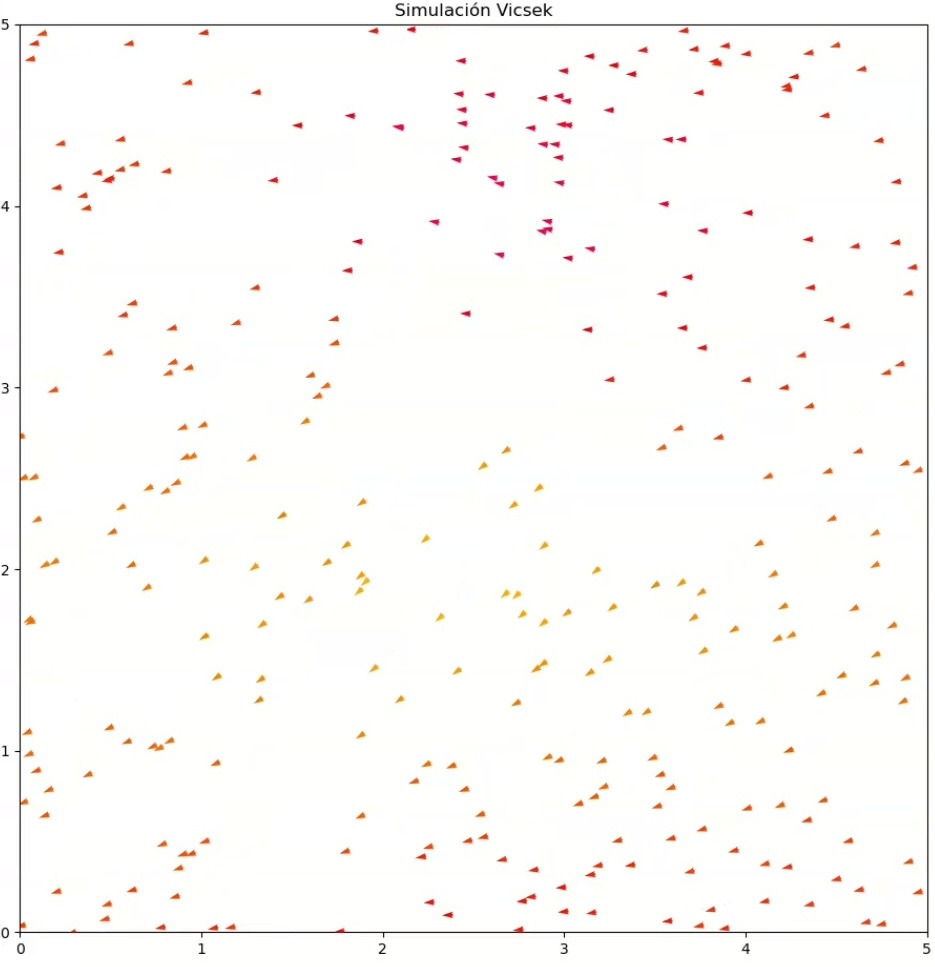
\includegraphics[width=6cm]{resources/animacion-eta-0.1.jpeg}
    \caption{Fotograma de la animación para $\eta=0.1$, $N=300$ y $L=5$.\\ \href{https://youtube.com/shorts/tTuYZXHlj-A}{Link} a la animación completa.}
    \label{animacion-eta-0.1}
\end{figure}

Luego, en la Fig.~\ref{animacion-eta-2} se presenta la simulación con un ruido intermedio ($\eta=2$), donde se observa un comportamiento más complejo, pues el sistema tiende a formar regiones alineadas, pero el ruido es suficiente para romper estas estructuras y dificultar el orden completo.\\

\begin{figure}[ht]
    \centering
    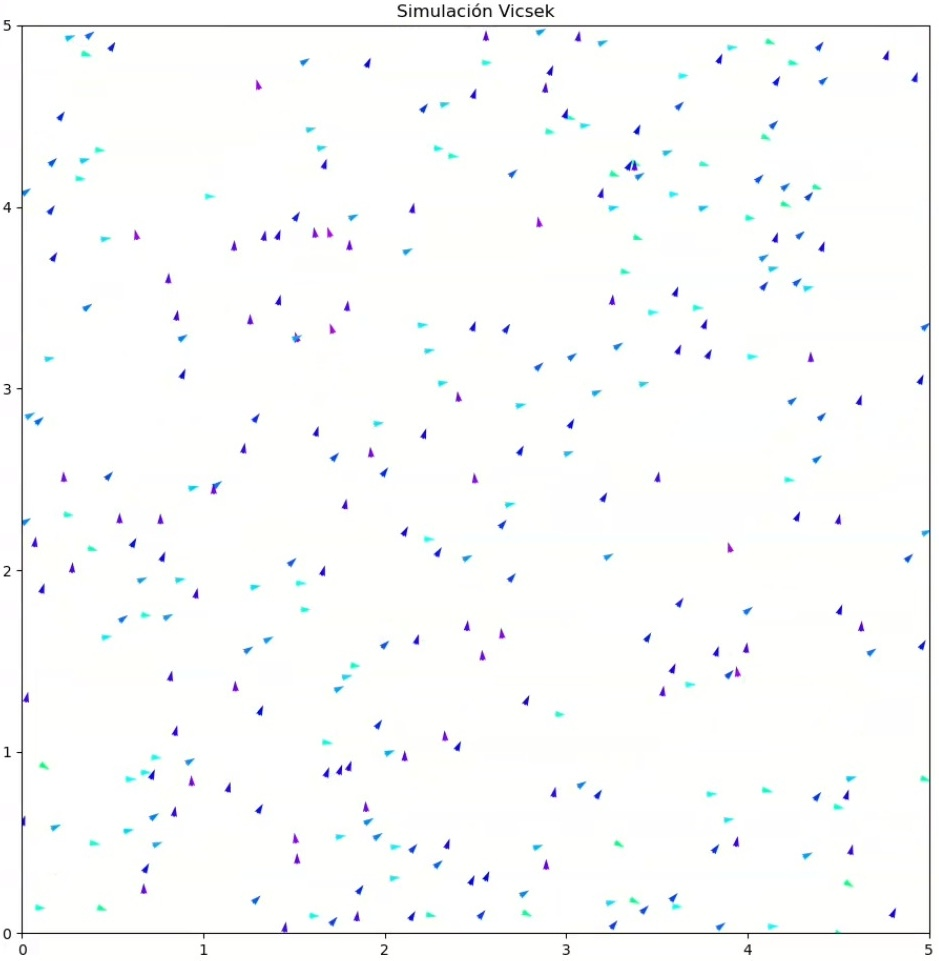
\includegraphics[width=6cm]{resources/animacion-eta-2.jpeg}
    \caption{Fotograma de la animación para $\eta=2$, $N=300$ y $L=5$.\\ \href{https://youtube.com/shorts/PRxFTmzgdxo}{Link} a la animación completa.}
    \label{animacion-eta-2}
\end{figure}

En la Fig.~\ref{animacion-eta-2pi}, se ilustra el caso de un ruido máximo ($\eta=6.28\approx 2\pi$). Bajo esta condición, las direcciones de las partículas son completamente aleatorias en cada paso temporal, lo que impide cualquier tipo de correlación a gran escala. El sistema se mantiene constantemente desordenado.\\

\begin{figure}[ht]
    \centering
    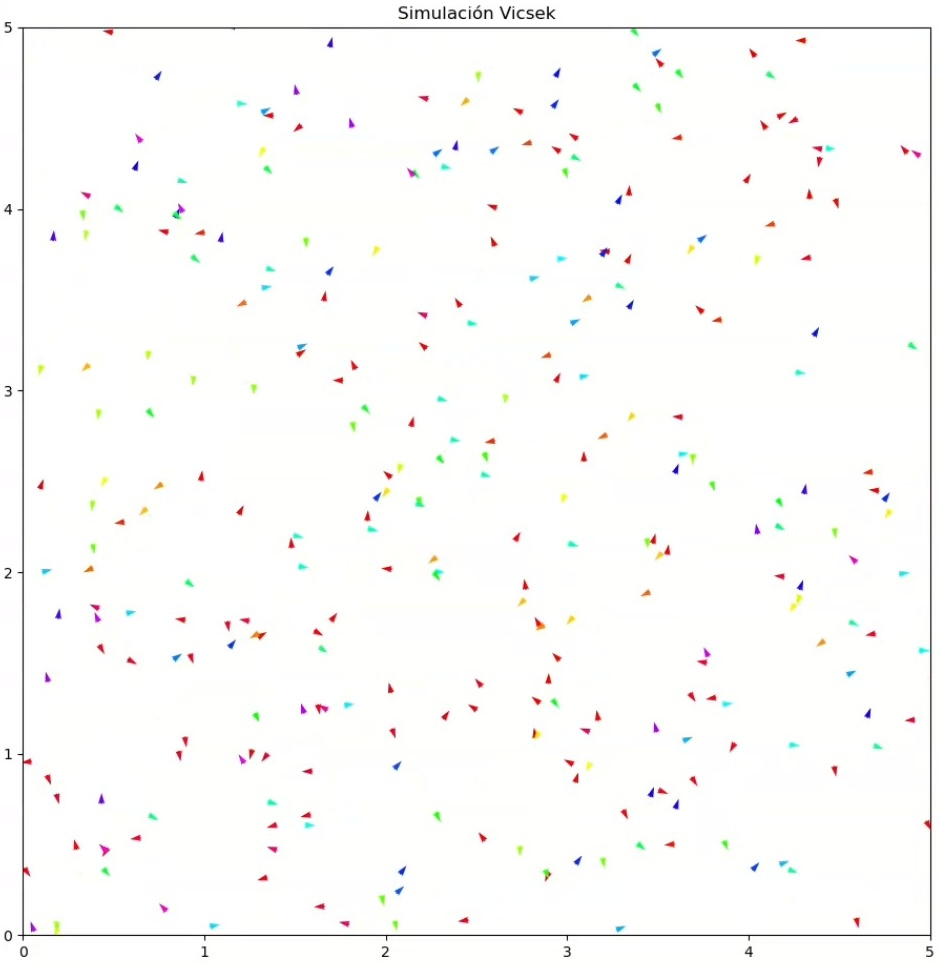
\includegraphics[width=6cm]{resources/animacion-eta-2pi.jpeg}
    \caption{Fotograma de la animación para $\eta\approx2\pi$, $N=300$ y $L=5$.\\ \href{https://youtube.com/shorts/hZ2bDILFapQ}{Link} a la animación completa.}
    \label{animacion-eta-2pi}
\end{figure}

En la Fig.~\ref{animacion-l-25}, se muestra además la simulación adicional en la que se incrementó el tamaño del sistema a $L=25$, manteniendo el resto de los parámetros constantes y $\eta=0.1$. En este caso, la densidad de partículas es menor, lo que implica que el alineamiento global se alcance de manera más lenta y menos homogénea. Las partículas tienden a agruparse en pequeños conjuntos que se desplazan en la misma dirección, pero la orientación general del sistema resulta menos definida que en el caso de mayor densidad.

\begin{figure}[ht]
    \centering
    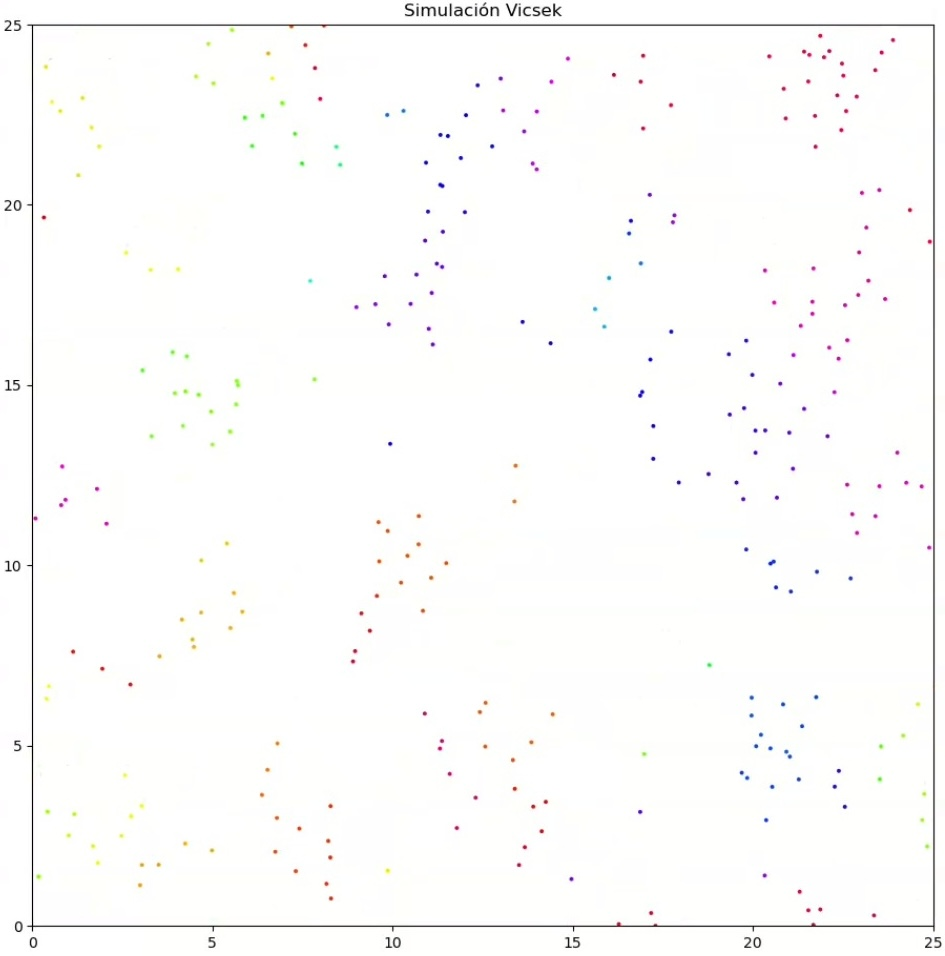
\includegraphics[width=6cm]{resources/animacion-l-25.jpeg}
    \caption{Fotograma de la animación para $\eta=0.1$, $N=300$ y $L=25$.\\ \href{https://www.youtube.com/shorts/jTQ0DtBW6Tg}{Link} a la animación completa.}
    \label{animacion-l-25}
\end{figure}

\subsection{Gráfico de la Evolución Temporal del Observable}

Para la simulación planteada en la Sección~\ref{evolucion-temporal-del-observable}, se obtuvieron los resultados mostrados en la Fig.~\ref{grafico-va-t}, donde se puede observar la evolución temporal del observable. En base al gráfico, se decidió tomar como tiempos para el cálculo promedio de $v_a$, es decir, el estado estacionario, los $t>0.3T$ siendo $T$ la cantidad de pasos. Se puede observar que a partir de dicho momento, todas las simulaciones para los distintos valores de $\eta$ alcanzan el estado estacionario.\\

\begin{figure}[ht]
    \centering
    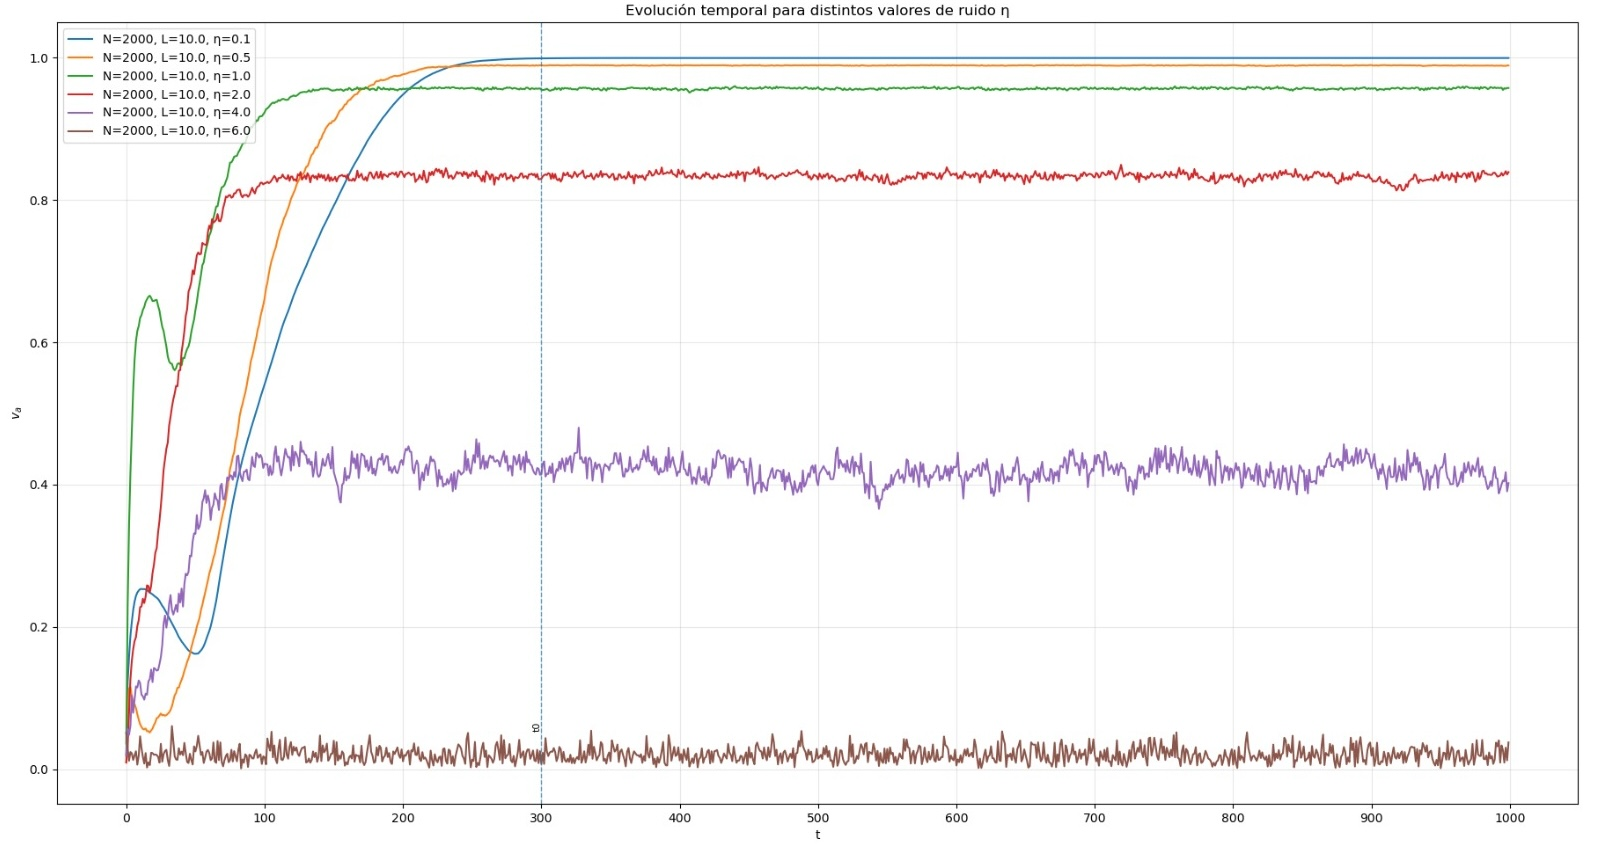
\includegraphics[width=12cm]{resources/grafico-va-t.jpeg}
    \caption{Gráfico del observable en función del tiempo.}
    \label{grafico-va-t}
\end{figure}

Para valores bajos de ruido ($\eta\in\{0.1,\;0.5\}$), el sistema alcanza rápidamente un estado ordenado con $v_a \approx 1$, mostrando una polarización casi perfecta y estable. En el caso intermedio ($\eta = 1.0$), el sistema llega a un valor estacionario de $v_a$ elevado pero menor que 1, reflejando un alineamiento parcial de las partículas con fluctuaciones visibles. Para ruidos mayores ($\eta = 2.0$), la polarización promedio disminuye hasta valores cercanos a $v_a \approx 0.8$, mostrando una cuota de orden colectivo y otra de desorden introducido por el ruido. Finalmente, para ruidos altos ($\eta\in\{4.0,\;6.0\}$), el sistema no logra organizarse: $v_a$ permanece en valores bajos y estables, alrededor de $0.4$ y casi $0$, respectivamente, lo que corresponde a un movimiento desordenado.\\

De esta manera, la evolución temporal muestra con claridad la transición desde un régimen ordenado a uno desordenado conforme aumenta el ruido $\eta$.

\subsection{Gráfico de la Relación entre el Ruido del Sistema y el Observable}

En la Fig.~\ref{grafico-va-eta} se muestra el gráfico correspondiente a la simulación desarrollada en la Sección~\ref{curva-input-vs-observable}. Se presentan los valores promedio del parámetro de orden $\overline{v_a}$ en función del ruido $\eta$, manteniendo constante la densidad $\rho=4$. Cada punto corresponde al promedio temporal del observable en régimen estacionario, mientras que las barras de error reflejan el desvío de $v_a(t)$ en dicho régimen, tal como se explicó anteriormente.\\

\begin{figure}[ht]
    \centering
    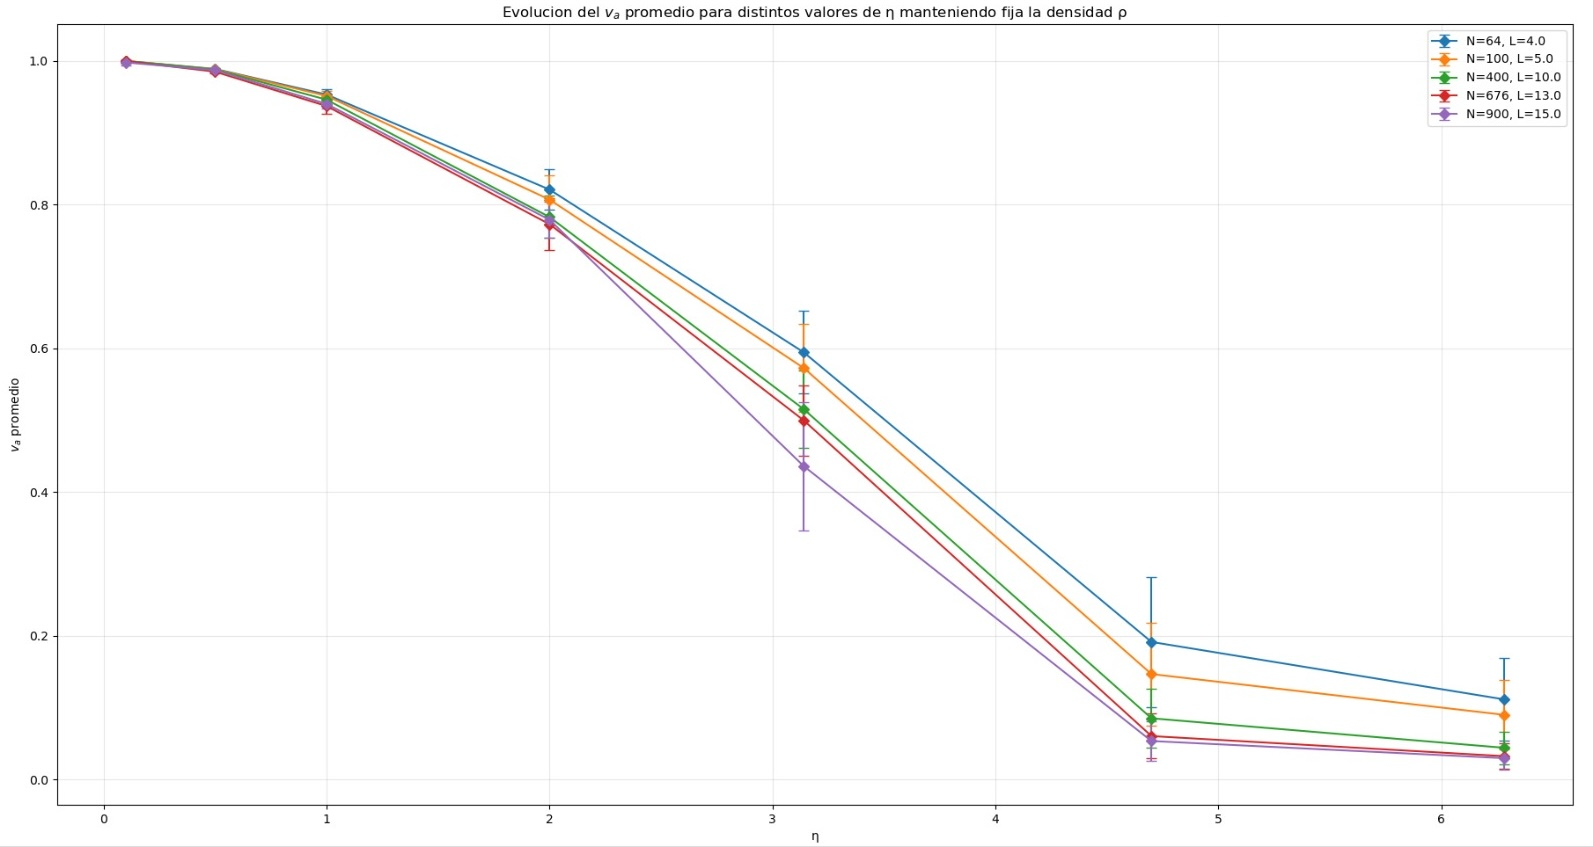
\includegraphics[width=12cm]{resources/grafico-va-eta.jpeg}
    \caption{Grafico de $v_a$ en función de $\eta$.}
    \label{grafico-va-eta}
\end{figure}

Se puede observar que para valores bajos de ruido ($\eta \le 1$), el sistema alcanza rápidamente un estado altamente ordenado con $\overline{v_a} \approx 1$, lo que indica un alineamiento casi perfecto de las partículas. A medida que el ruido aumenta, la polarización global disminuye progresivamente, señalando la pérdida de coherencia en la dirección de movimiento de las partículas.\\

Luego, para ruidos grandes ($\eta \ge 5$), el valor del parámetro de orden se aproxima a cero, reflejando un comportamiento completamente desordenado en el que las partículas se mueven en direcciones aleatorias.\\

En la Fig.~\ref{grafico-va-rho} se presenta el resultado de las simulaciones adicionales expresadas en la Sección~\ref{evolucion-temporal-del-observable}, variando la cantidad de partículas $N$ y, por lo tanto, la densidad. Cada punto muestra el valor promedio del parámetro de orden $\overline{v_a}$ en régimen estacionario, con sus respectivas barras de error.\\

\begin{figure}[ht]
    \centering
    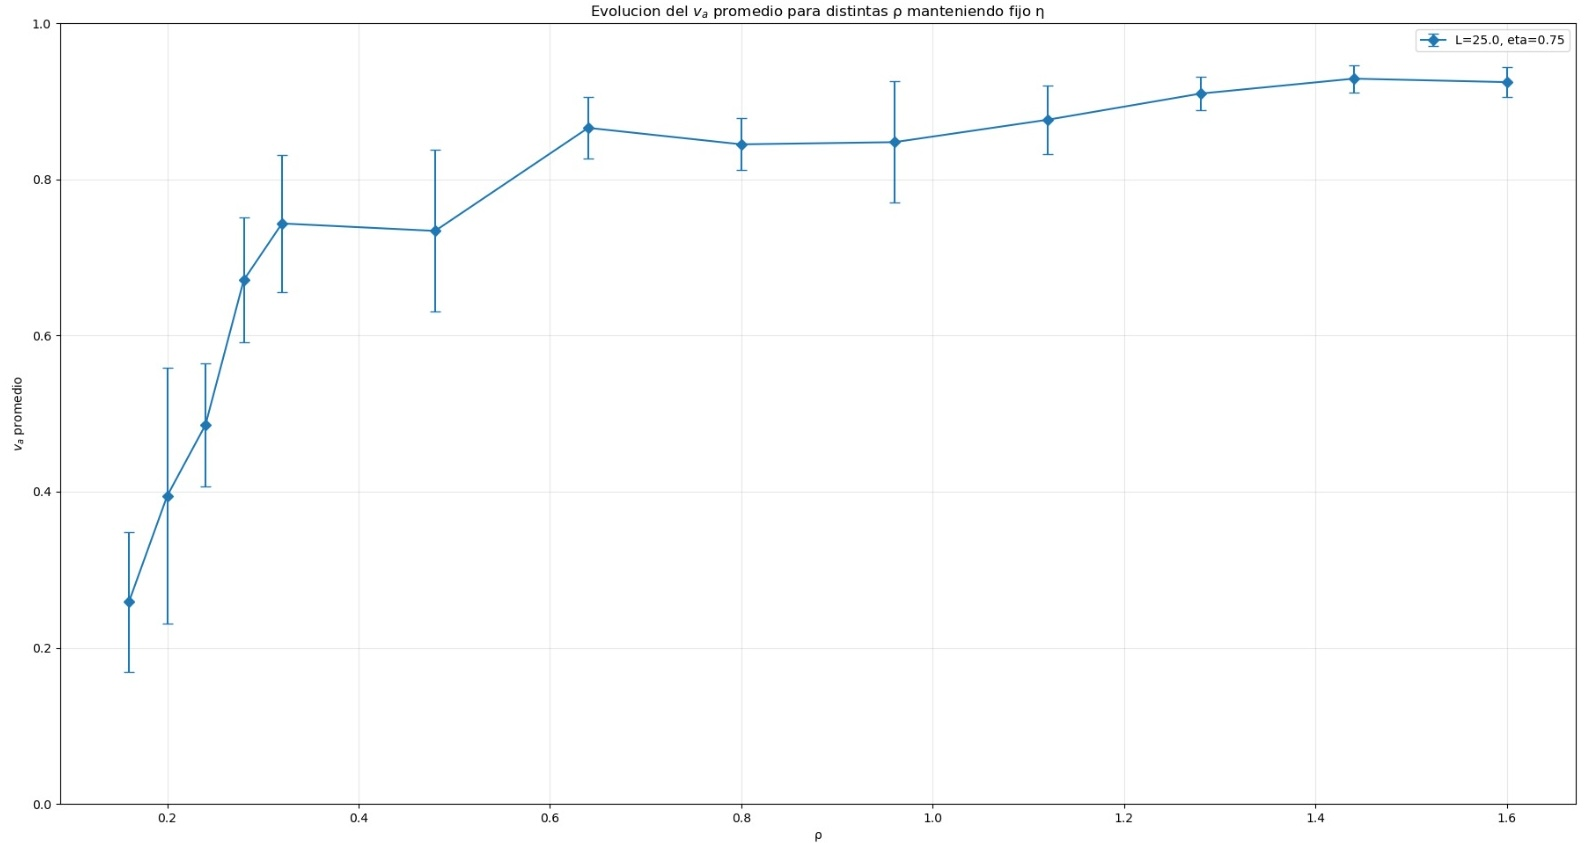
\includegraphics[width=12cm]{resources/grafico-va-rho.jpeg}
    \caption{Evolución del parámetro de orden promedio $\overline{v_a}$ en función de la densidad $\rho$, para $L=25$ y $\eta=0.75$.}
    \label{grafico-va-rho}
\end{figure}

Se observa un comportamiento creciente de la polarización promedio con la densidad del sistema. Para densidades bajas ($\rho < 0.3$), el sistema presenta un orden reducido ($\overline{v_a} \le 0.4$) y fuertes fluctuaciones, reflejadas en las barras de error más amplias. A medida que aumenta la densidad, el alineamiento colectivo mejora rápidamente y $\overline{v_a}$ crece de forma sostenida, superando valores de $0.8$ para $\rho \ge 0.6$.\\

Finalmente, para densidades altas ($\rho > 1$), el sistema alcanza un régimen de fuerte alineamiento global con $\overline{v_a} \approx 0.9$, manteniéndose estable incluso frente a las perturbaciones del ruido. Esto muestra que una mayor densidad favorece en cierto punto el orden colectivo, al incrementar la cantidad de interacciones promedio entre partículas dentro del radio de interacción $r_c$. \\

\subsection{Gráfico de la Interacción Tipo Votante}

Para la interacción de tipo votante, primero se animaron las tres simulaciones especificadas en la Sección~\ref{interaccion-tipo-votante}. En la Fig.~\ref{animacion-votante-n-300}, se puede observar el primer caso planteado donde el ruido $\eta$ es cero.  Si bien el orden del sistema tarda en establecerse a diferencia de las animaciones de la Sección~\ref{simulaciones-para-animaciones}, se termina llegando a una eventual polarización total.\\

\begin{figure}[ht]
    \centering
    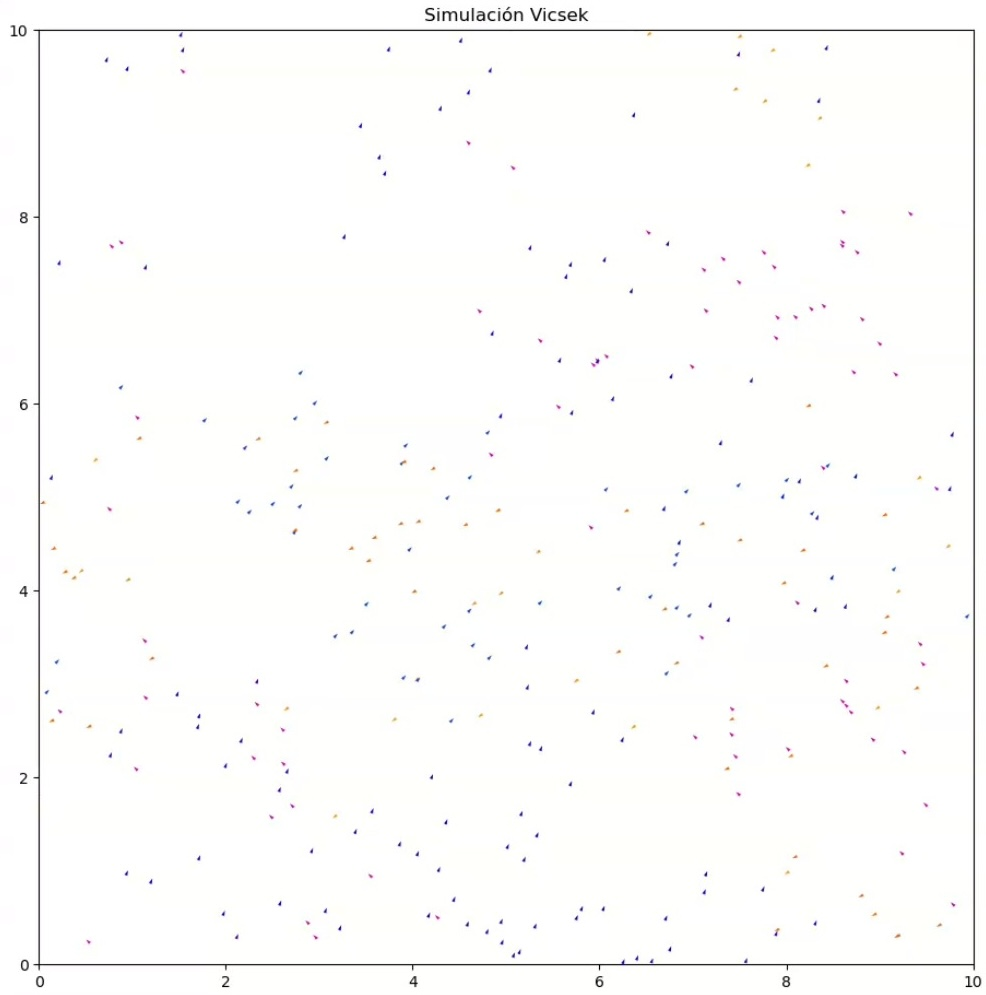
\includegraphics[width=6cm]{resources/animacion-votante-n-300.jpeg}
    \caption{Fotograma de la animación de tipo votante para $N=300$, $L=10$ y $\eta=0$.\\ 
    \href{https://www.youtube.com/shorts/W_7f7Aq2uGs}{Link} a la animación completa.}
    \label{animacion-votante-n-300}
\end{figure}

En la animación presentada en la Fig.~\ref{animacion-votante-n-300-eta} se agrega el ruido $\eta=0.5$, que si bien es bajo, se puede apreciar que es suficiente para que el sistema nunca alcance un orden total, al menos para la cantidad de pasos $T$ observados. Esto muestra la implicancia que tienen aunque sean pequeñas perturbaciones en la polarización de todo el sistema y cómo se entorpece el alcance de un estado estacionario, como sí sucedía en las secciones anteriores.\\

\begin{figure}[ht]
    \centering
    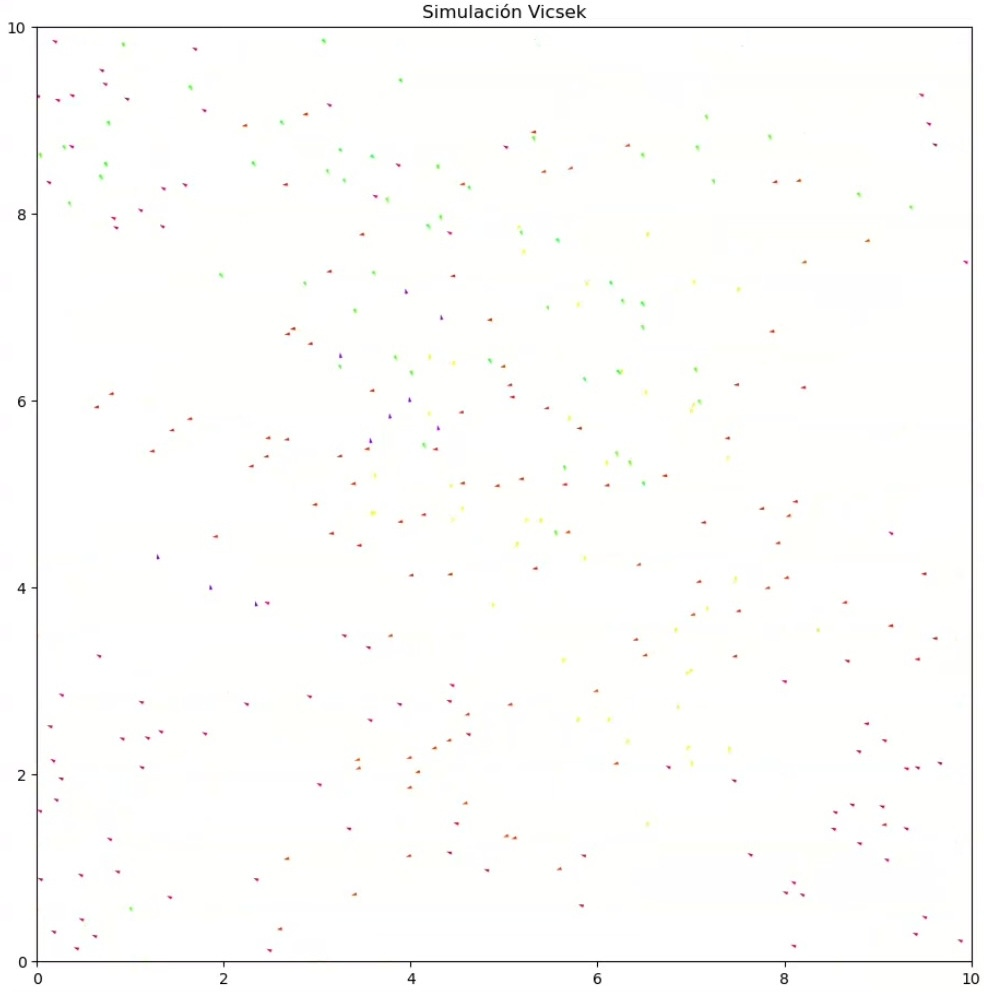
\includegraphics[width=6cm]{resources/animacion-votante-n-300-eta.jpeg}
    \caption{Fotograma de la animación de tipo votante para $N=300$, $L=10$ y $\eta=0.5$.\\ 
    \href{https://www.youtube.com/shorts/x6ymonK0mbM}{Link} a la animación completa.}
    \label{animacion-votante-n-300-eta}
\end{figure}

En el tercer caso presentado, se obtuvo la animación mostrada en la Fig.~\ref{animacion-votante-n-2000}, donde se puede ver el impacto de un aumento notable en la densidad $\rho$ al incrementar la cantidad de partículas $N$. Aunque nuevamente se tomó un ruido nulo ($\eta = 0$), la dinámica observada difiere del primer escenario con menor cantidad de partículas. A medida que la densidad crece, las interacciones locales se vuelven más frecuentes y las direcciones de las partículas cambian constantemente, lo que dificulta que el sistema logre un orden global.\\

\begin{figure}[ht]
    \centering
    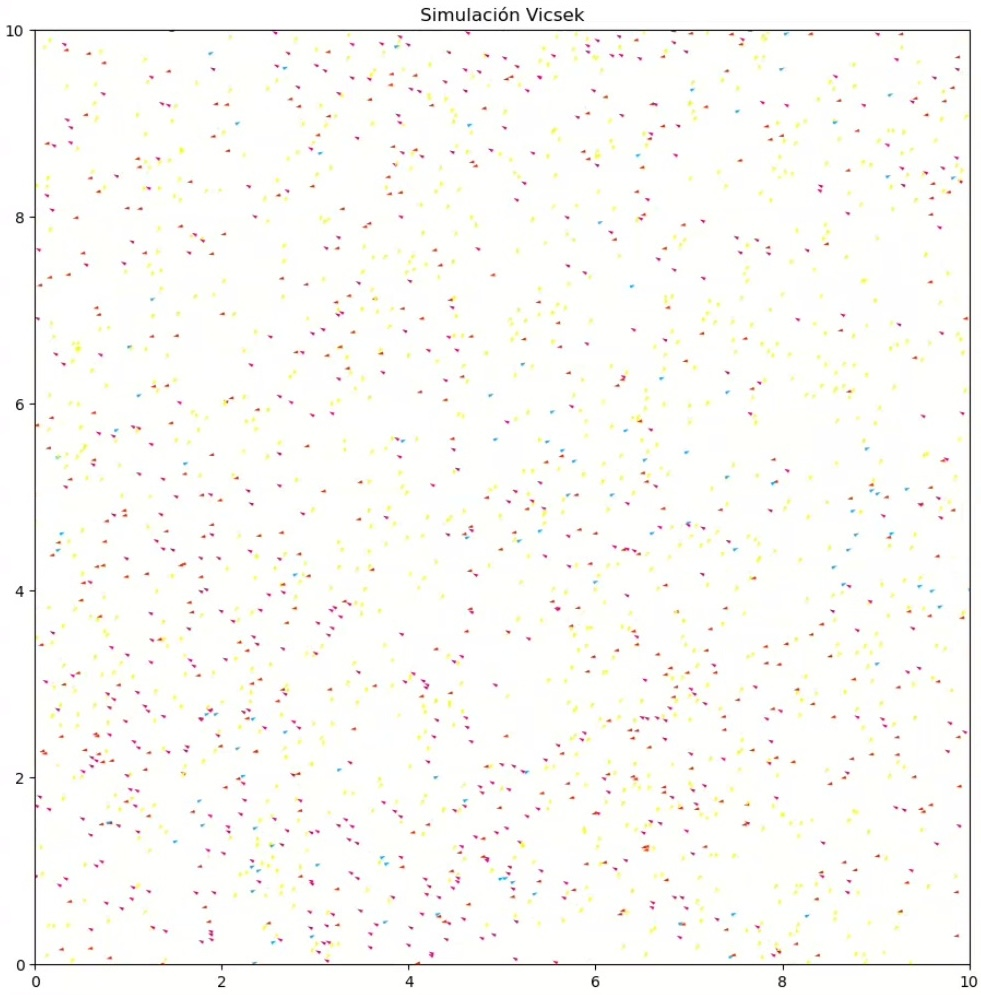
\includegraphics[width=6cm]{resources/animacion-votante-n-2000.jpeg}
    \caption{Fotograma de la animación de tipo votante para $N=2000$, $L=10$ y $\eta=0$.\\ 
    \href{https://www.youtube.com/shorts/ISQq8_p_pDQ}{Link} a la animación completa.}
    \label{animacion-votante-n-2000}
\end{figure}

Esto demuestra que, bajo la regla tipo votante, un mayor número de partículas no necesariamente favorece el orden total, sino que, por el contrario, la abundancia de interacciones hace que la propagación de orientaciones aleatorias entre vecinos genere fluctuaciones persistentes que impiden la consolidación de una única dirección dominante en todo el sistema.\\

Para observar estos resultados y analizar con mayor claridad el efecto del ruido, se realizó el gráfico para la segunda tanda de simulaciones porpuestas en la Sección~\ref{interaccion-tipo-votante}. En la Fig.~\ref{grafico-votante-va} se muestran los resultados de la evolución temporal del parámetro de orden $v_a(t)$ para la regla de interacción tipo votante.\\

\begin{figure}[ht]
    \centering
    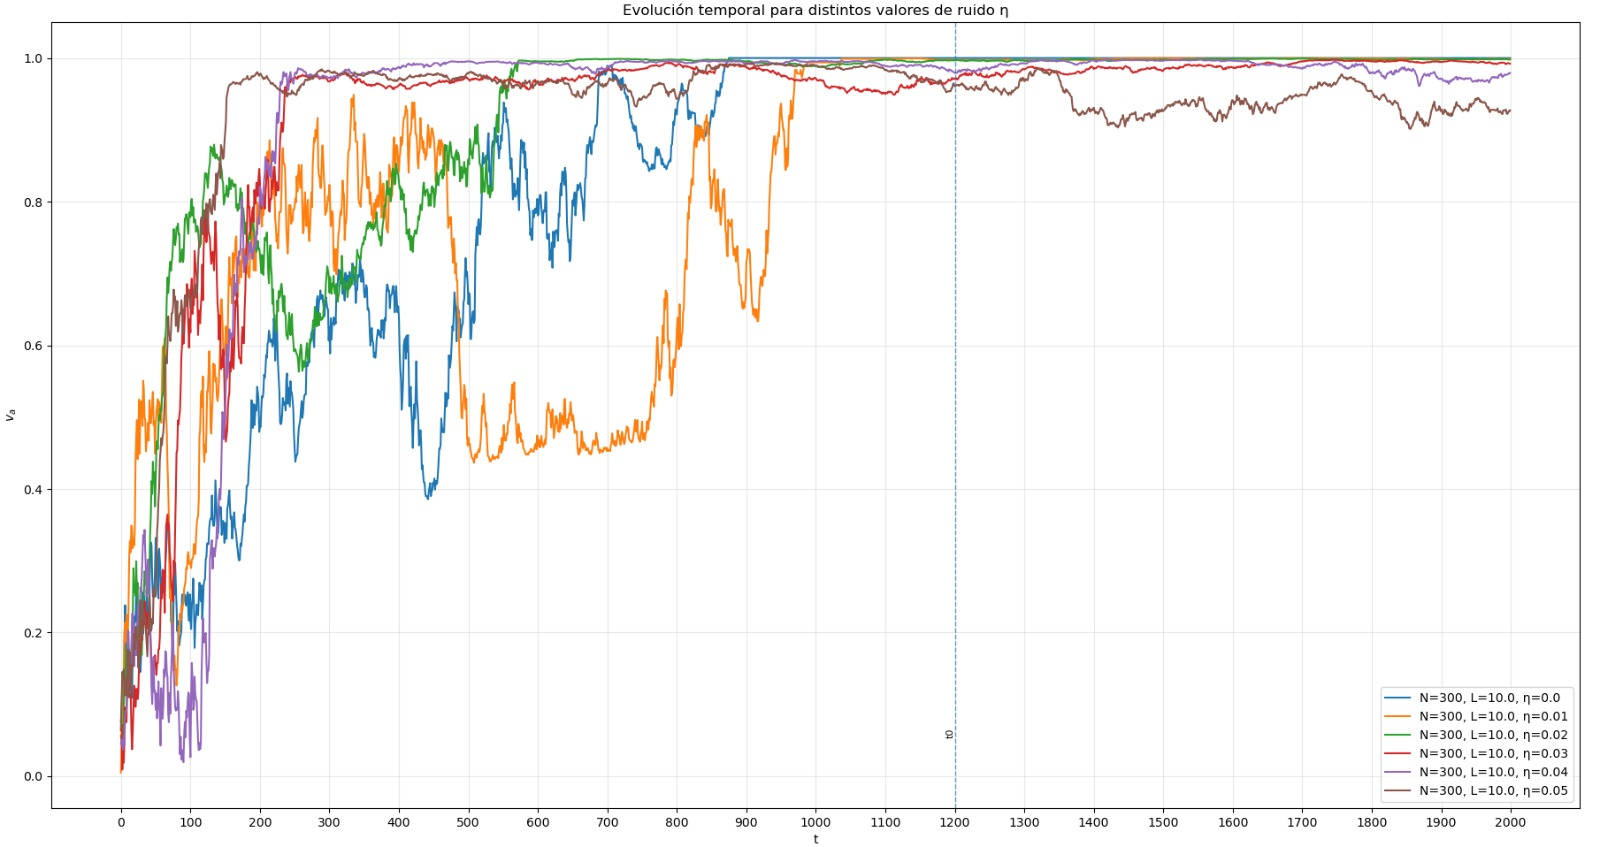
\includegraphics[width=12cm]{resources/grafico-votante-va.jpeg}
    \caption{Grafico de $v_a$ en función de $\eta$ para la interacción de tipo votante.}
    \label{grafico-votante-va}
\end{figure}

Si se compara este gráfico con el de la Fig.~\ref{grafico-va-t}, se puede 
observar cómo el estado estacionario tarda mucho más en alcanzarse. Además, es posible observar al igual que en las simulaciones previas que para el mayor valor de $\eta$, el estado estacionario es más inestable a pesar de encontrarse en valores de $v_a(t)$ cercanos a $1$.\\

En base a estos resultados, se tomó como criterio de régimen estacionario $t > 0.6T$, a pesar de las especificaciones mencionadas previamente.  Teniendo esto en cuenta, se realizó la tercera tanda de simulaciones planteadas en la Sección~\ref{interaccion-tipo-votante} con un ruido igual a cero. El gráfico obtenido en la Fig.~\ref{grafico-votante} muestra la evolución de la polarización promedio $\overline{v_a}$ en función de la densidad $\rho$, variando la cantidad de partículas $N$ para un tamaño de celda fijo $L=10$.\\

\begin{figure}[ht]
    \centering
    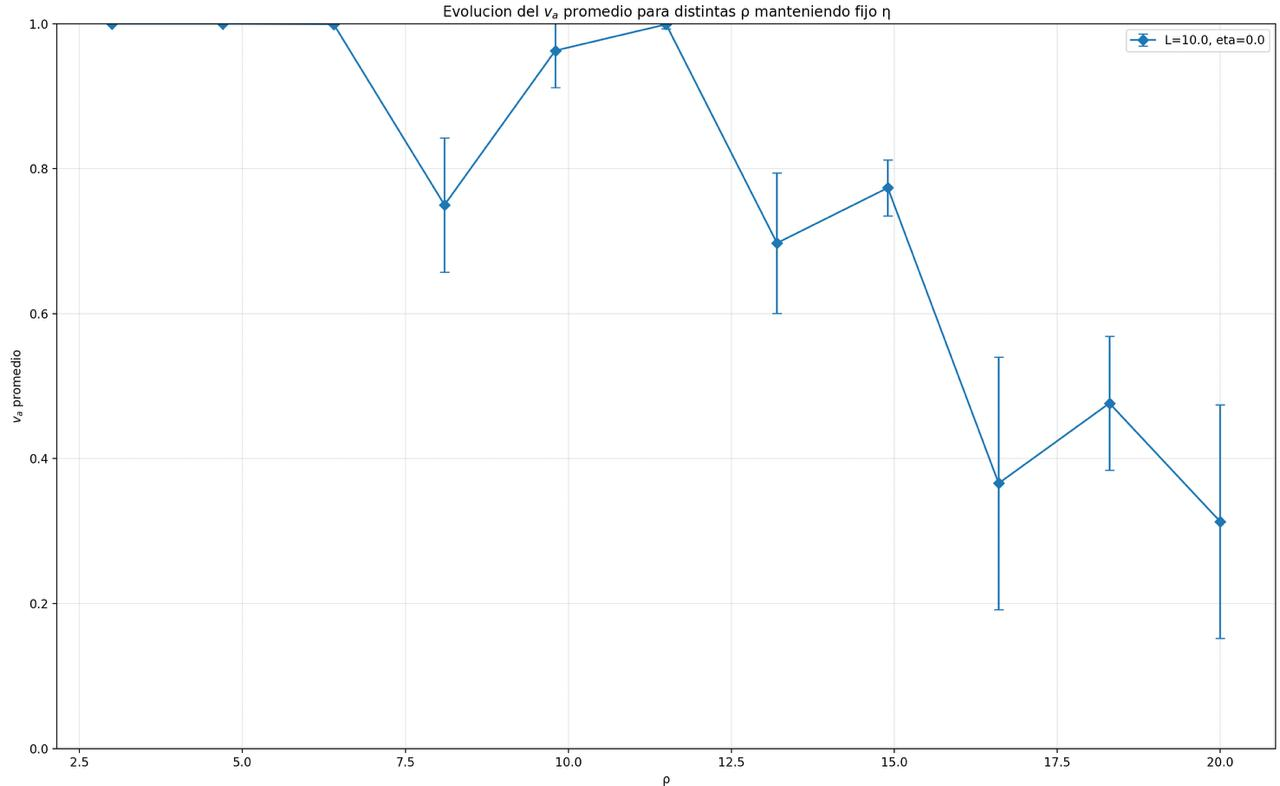
\includegraphics[width=12cm]{resources/grafico-votante.jpeg}
    \caption{Parámetro de orden promedio $\overline{v_a}$ en función de la densidad $\rho$ para la interacción tipo votante con $L=10$ y $\eta=0$.}
    \label{grafico-votante}
\end{figure}

En este escenario, se observa que para densidades bajas el sistema tiende a presentar valores altos de polarización, aunque con una dispersión considerable. A medida que $\rho$ aumenta, las fluctuaciones se vuelven más evidentes y el valor promedio de $\overline{v_a}$ deja de crecer de forma sistemática, llegando incluso a mostrar caídas en regiones intermedias. Esto refleja que, bajo la dinámica tipo votante, el orden colectivo depende fuertemente de la configuración inicial y de las elecciones aleatorias de vecinos, a diferencia del modelo de Vicsek original, donde el promedio sobre varios vecinos favorece la estabilidad del alineamiento.

\section{Conclusión}

En este trabajo se implementó y analizó el modelo de Vicsek, un sistema que permite estudiar la dinámica de modelos de partículas autopropulsadas en dos dimensiones.\\

Los resultados obtenidos muestran que el parámetro de orden $v_a$ depende en gran medida del nivel de ruido $\eta$. Para valores bajos de $\eta$, el sistema alcanza rápidamente un estado de orden global, mientras que al incrementar el ruido se pudo observar una pérdida progresiva del orden hasta llegar a un régimen de completo desorden. Esto pudo ser verificado tanto en las animaciones como en la evolución temporal del observable y en la curva $\overline{v_a}$ en función de $\eta$.\\ 

Asimismo, el análisis de la densidad $\rho$ mostró que al aumentar la cantidad de partículas en el sistema, manteniendo fijo el tamaño de la celda, se favorece la formación de un mayor orden colectivo. En este contexto, la polarización promedio se incrementa y las fluctuaciones disminuyen, demostrando la importancia de la densidad como factor clave en la estabilidad del sistema.\\

Por último, la variante de interacción tipo votante permitió contrastar el modelo original con una regla de actualización diferente. En este esquema, el sistema no alcanza un régimen estacionario estable si se dispone de aunque sea una pequeña cuota de ruido, y sólo en el caso particular de $\eta=0$ se observa un orden más consistente, aunque con ciertas fluctuaciones más marcadas que en el caso previo.\\

En conclusión, el estudio realizado evidencia cómo reglas de interacción locales y parámetros globales como el ruido y la densidad determinan la aparición o desaparición de un orden colectivo o polarización total en sistemas de partículas autopropulsadas.

\end{document}


